\thispagestyle{fancy}
\chapter{Result And Analysis} \label{ch:result_and_analysis}
\section*{\centering Chapter \thechapter}
\section*{\centering Result And Analysis}


\section{Performance Measures} \label{sec:performance_measures}
There are a lot of different types of parameters to evaluate the performance of machine learning models. In case of the classification models Accuracy score, F1 score, Recall score, Precision score and total area under ROC curve used for performance evaluation.

\subsection{Accuracy Score}\label{subsec:accuracy_score}
The accuracy score is a fraction of the correct prediction by model with respect to total predictions by model. It can be represented by following formula:

\begin{equation}\label{eq:accuracy_score}
  Accuracy = \frac{TP+TN}{TP+TN+FP+FN}
\end{equation}
\myequations{Accuracy Score}

\subsection{Precision score}\label{subsec:precision_score}
The precision score is a fraction of the correct positive predictions with respect to all positive predictions of the model. Higher precision scores result in fewer false positive predictions. It can be represented by following formula:

\begin{equation}\label{eq:precision_score}
  Precision = \frac{TP}{TP+FP}
\end{equation}
\myequations{Precision Score}

\subsection{Recall score}\label{subsec:recall_score}
The recall score is the fraction of correct positive predictions with respect to all predictions of the class. It can be represented by following formula:

\begin{equation}\label{eq:recall_score}
  Recall = \frac{TP}{TP+FN}
\end{equation}
\myequations{Recall Score}

\subsection{F1 score}\label{subsec:f1_score}
The F1 score is the weighted average of the recall score and precision score of the model. F1 scores are more reliable than accuracy scores in case of biased or uneven dataset. It can be represented by following formula:

\begin{equation}\label{eq:f1_score}
  F1 = 2 \cdot \frac{Recall \cdot Precision}{Recall + Precision}
\end{equation}
\myequations{F1 Score}

F1 score can also be represented as
$F1 = \frac{TP}{TP+\frac{1}{2}(FP+FN)}$

\subsection{AUC ROC score}\label{subsec:auc_roc_score}
The ROC is a classifier's predictive quality that compares and visualizes the trade-off between the model's sensitivity and specificity. In graphical format, the area under it gives a relationship between false positives and true positives. The higher these areas are, the better the predictive quality of the model.

\subsection{Prediction Time}\label{subsec:prediction_time}
Prediction times are nothing but the amount of time required by the classifier to make predictions for certain testing datasets. A model with a lower prediction time is desirable.

\subsection{Performance Evaluation Methodology} \label{subsec:performance_evaluation_methodology}
Performance scores are calculated with performance evaluation metrics and average prediction time. The models are ranked based on performance scores.

Weighted sums of the ranks are stored for the selection process. Weightage is predefined. It lies between 0 to 1, and it is directly proportional to the significance of the metric. For example, in situations where speed is more important than accuracy, prediction time is given higher weightage than accuracy metrics.

In the proposed system lowest scoring model is selected as the ideal model.

\section{Dataset Description} \label{sec:dataset_description}
The goal of the project is to detect the presence of arrhythmia from ECG signals accurately and faster than the traditional approach. For this task, a well-known open-access database MIT-BIH Arrhythmia Training and Testing Dataset are used. Both datasets are divided into four equal parts randomly and used for training and testing respectively. Each training set contains 21888 signals and the testing set contains 5473 signals.

\section{Performance Evaluation} \label{sec:performance_evaluation}
The datasets obtained from the MIT-BIH training dataset showed significant similarities in performance evaluation. All four datasets showed higher performance metrics for SVM classifiers. The prediction time required by SVM and KNN was significantly higher than other classifiers. The desired result can be tweaking ranking parameters. The performance results of the models as shown in figure %\ref{fig:perfromance_results}

% ************** Performance of models trained on dataset 1, 2, 3, and 4 tabular **************
% ***************************************** Dataset 1 *****************************************
\begin{table}[H]
  \centering
  \caption{Performance of models trained on Dataset 1}\label{tab:performance_of_models_trained_on_dataset_1}
  \begin{tabular}{|p{5em}|C{3em}|C{3em}|C{3em}|C{3em}|C{3em}|}
    \hline
    \textbf{Metric}    & \textbf{KNN} & \textbf{DT} & \textbf{MLP} & \textbf{RF} & \textbf{SVM}   \\
    \hline
    \textbf{Accuracy}  & 96.72        & 94.46       & 96.89        & 97.33       & \textbf{97.40} \\
    \textbf{F1}        & 89.71        & 83.43       & 90.05        & 91.30       & \textbf{91.69} \\
    \textbf{Precision} & 92.53        & 81.86       & 94.71        & 97.95       & \textbf{96.43} \\
    \textbf{Recall}    & 87.06        & 85.06       & 85.84        & 85.50       & \textbf{87.40} \\
    \textbf{ROC}       & 92.84        & 90.68       & 92.45        & 92.57       & \textbf{93.38} \\
    \textbf{Time(s)}   & 0.457        & 0.001       & 0.002        & 0.015       & \textbf{0.297} \\
    \hline
  \end{tabular}
\end{table}

% ***************************************** Dataset 2 *****************************************
\begin{table}[H]
  \centering
  \caption{Performance of models trained on Dataset 2}\label{tab:performance_of_models_trained_on_dataset_2}
  \begin{tabular}{|p{5em}|C{3em}|C{3em}|C{3em}|C{3em}|C{3em}|}
    \hline
    \textbf{Metric}    & \textbf{KNN} & \textbf{DT} & \textbf{MLP} & \textbf{RF} & \textbf{SVM}   \\
    \hline
    \textbf{Accuracy}  & 96.83        & 95.04       & 96.69        & 97.09       & \textbf{97.46} \\
    \textbf{F1}        & 90.28        & 85.50       & 89.73        & 90.75       & \textbf{92.15} \\
    \textbf{Precision} & 94.25        & 84.90       & 94.73        & 98.60       & \textbf{96.79} \\
    \textbf{Recall}    & 86.63        & 86.09       & 85.23        & 84.05       & \textbf{87.93} \\
    \textbf{ROC}       & 92.77        & 91.48       & 92.13        & 91.90       & \textbf{93.66} \\
    \textbf{Time(s)}   & 0.435        & 0.001       & 0.003        & 0.014       & \textbf{0.295} \\
    \hline
  \end{tabular}
\end{table}

% ***************************************** Dataset 3 *****************************************
\begin{table}[H]
  \centering
  \caption{Performance of models trained on Dataset 3}\label{tab:performance_of_models_trained_on_dataset_3}
  \begin{tabular}{|p{5em}|C{3em}|C{3em}|C{3em}|C{3em}|C{3em}|}
    \hline
    \textbf{Metric}    & \textbf{KNN} & \textbf{DT} & \textbf{MLP} & \textbf{RF}    & \textbf{SVM} \\
    \hline
    \textbf{Accuracy}  & 97.07        & 94.64       & 96.41        & \textbf{97.22} & 97.44        \\
    \textbf{F1}        & 90.93        & 84.30       & 89.34        & \textbf{91.21} & 92.00        \\
    \textbf{Precision} & 95.82        & 83.81       & 90.13        & \textbf{98.37} & 97.81        \\
    \textbf{Recall}    & 86.53        & 84.80       & 88.57        & \textbf{85.02} & 86.85        \\
    \textbf{ROC}       & 92.87        & 90.73       & 93.29        & \textbf{92.36} & 93.22        \\
    \textbf{Time(s)}   & 0.404        & 0.001       & 0.002        & \textbf{0.017} & 0.293        \\
    \hline
  \end{tabular}
\end{table}

% ***************************************** Dataset 4 *****************************************
\begin{table}[H]
  \centering
  \caption{Performance of models trained on Dataset 4}\label{tab:performance_of_models_trained_on_dataset_4}
  \begin{tabular}{|p{5em}|C{3em}|C{3em}|C{3em}|C{3em}|C{3em}|}
    \hline
    \textbf{Metric}    & \textbf{KNN} & \textbf{DT} & \textbf{MLP} & \textbf{RF} & \textbf{SVM}   \\
    \hline
    \textbf{Accuracy}  & 96.84        & 94.99       & 95.34        & 96.88       & \textbf{97.15} \\
    \textbf{F1}        & 90.52        & 85.73       & 85.01        & 90.37       & \textbf{91.39} \\
    \textbf{Precision} & 95.71        & 85.91       & 97.83        & 98.65       & \textbf{97.41} \\
    \textbf{Recall}    & 85.86        & 85.55       & 75.15        & 83.37       & \textbf{86.07} \\
    \textbf{ROC}       & 92.52        & 91.28       & 87.40        & 91.56       & \textbf{92.79} \\
    \textbf{Time(s)}   & 0.452        & 0.001       & 0.002        & 0.014       & \textbf{0.294} \\
    \hline
  \end{tabular}
\end{table}

% ************* Performance of models trained on dataset 1, 2, 3, and 4 graphical *************
\begin{figure}[H]
  % ***************************************** Dataset 1 *****************************************
  \begin{subfigure}{.5\columnwidth}
    \centering
    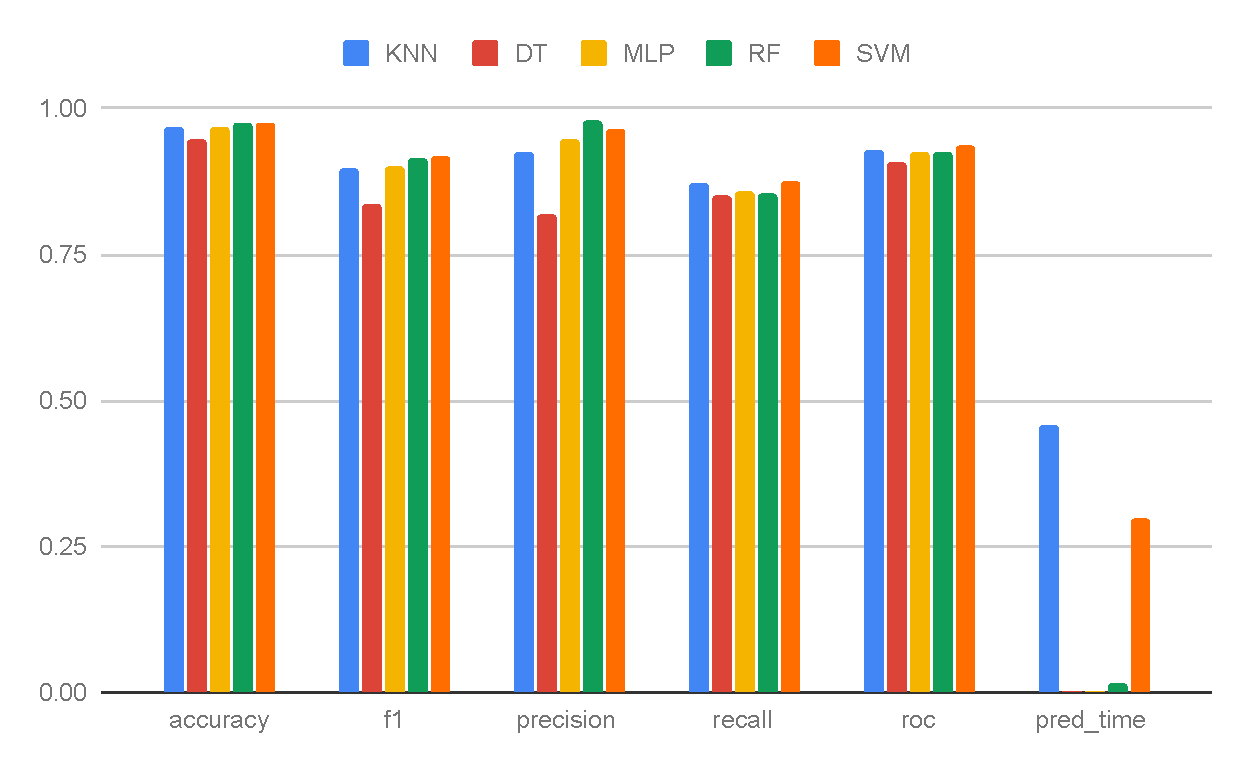
\includegraphics[width=0.9\columnwidth]{media/data/performance/perf_ds_1.pdf}
    \caption{Dataset 1}
    \label{fig:perfromance_results_dataset_1}
  \end{subfigure}%
  % ***************************************** Dataset 2 *****************************************
  \begin{subfigure}{.5\columnwidth}
    \centering
    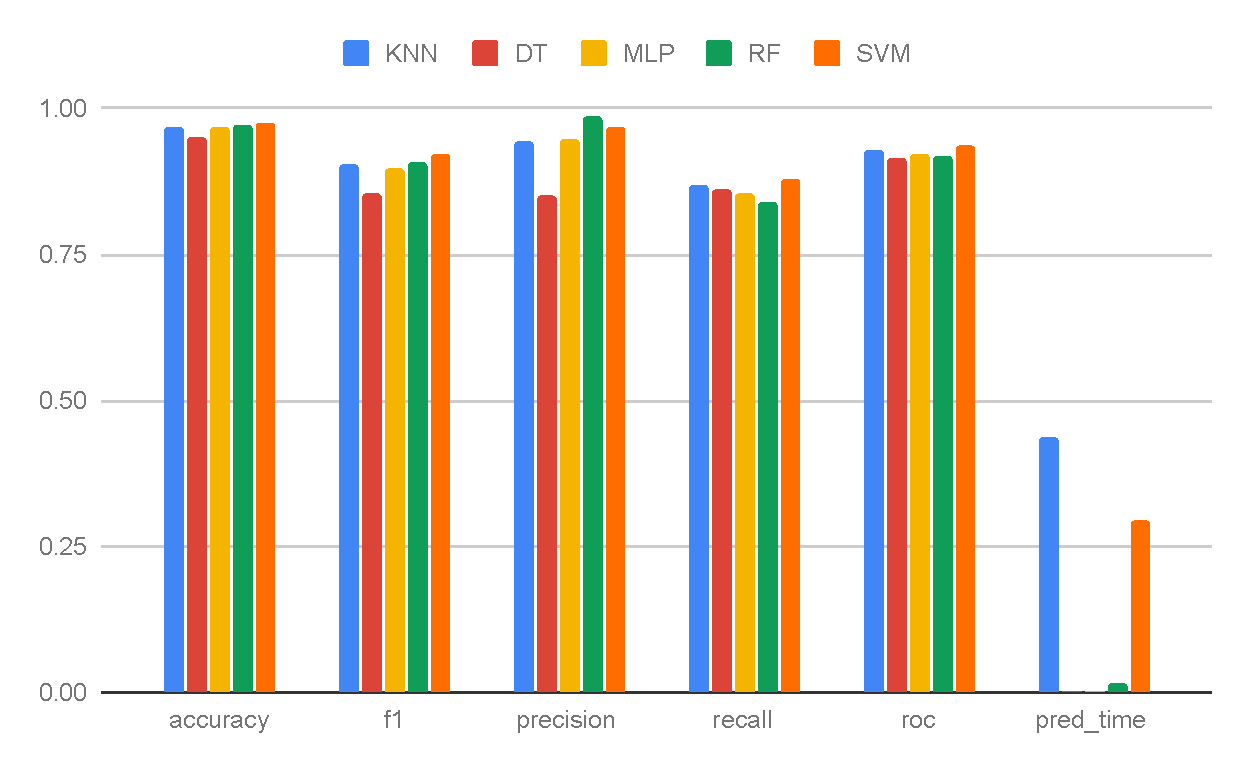
\includegraphics[width=0.9\columnwidth]{media/data/performance/perf_ds_2.pdf}
    \caption{Dataset 2}
    \label{fig:perfromance_results_dataset_2}
  \end{subfigure}\\%
  % ***************************************** Dataset 3 *****************************************
  \begin{subfigure}{.5\columnwidth}
    \centering
    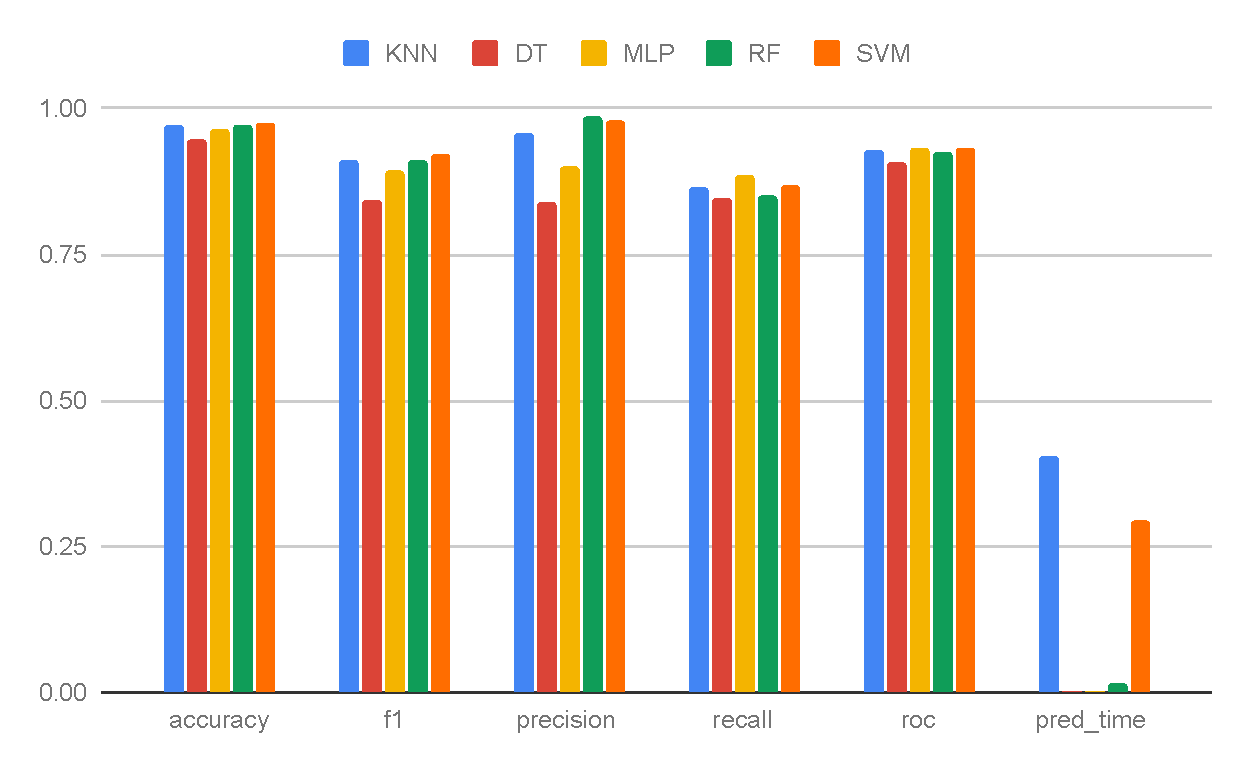
\includegraphics[width=0.9\columnwidth]{media/data/performance/perf_ds_3.pdf}
    \caption{Dataset 3}
    \label{fig:perfromance_results_dataset_3}
  \end{subfigure}%
  % ***************************************** Dataset 4 *****************************************
  \begin{subfigure}{.5\columnwidth}
    \centering
    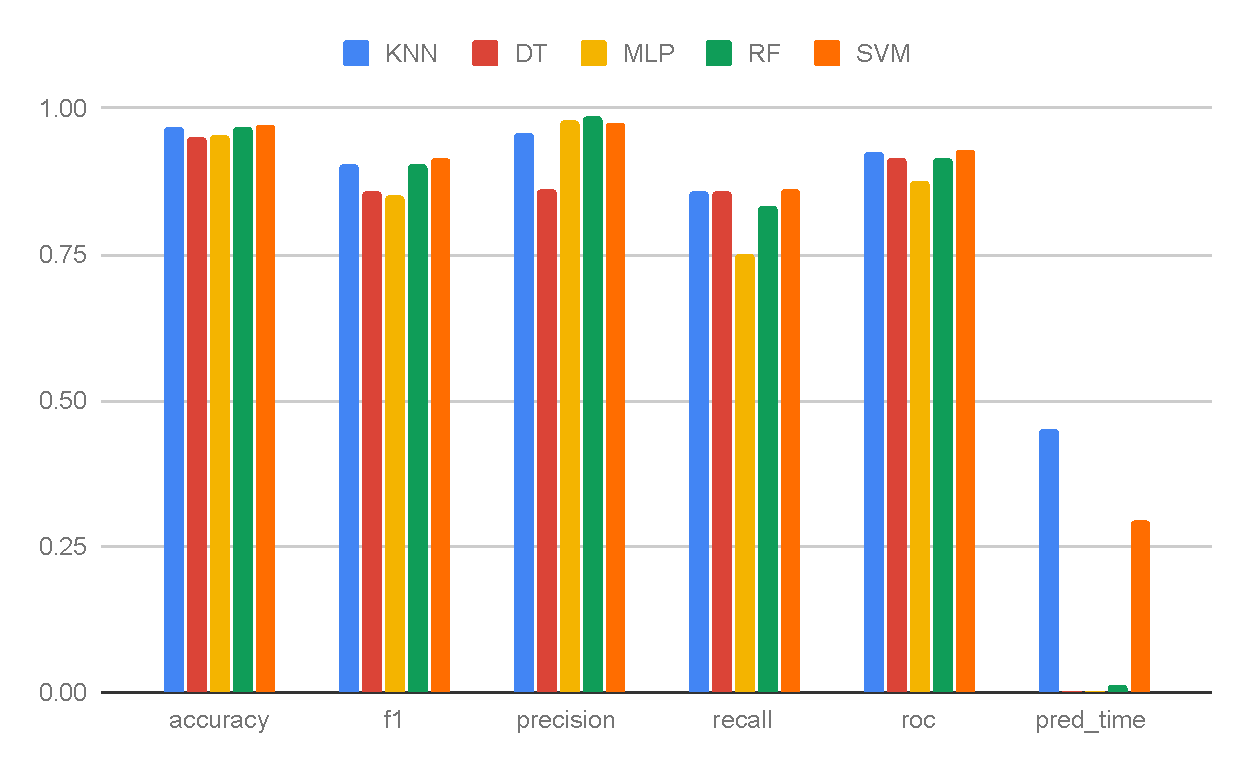
\includegraphics[width=0.9\columnwidth]{media/data/performance/perf_ds_4.pdf}
    \caption{Dataset 4}
    \label{fig:perfromance_results_dataset_4}
  \end{subfigure}
  \caption{Perfromance Results}
  \label{fig:perfromance_results}
\end{figure}

\section{Cross Performance Evaluation} \label{sec:cross_performance_evaluation}

Models tested against other datasets show a slight difference in performance. This difference suggests that the models are capable of performing general predictions. These general tasks can be performed with a small efficiency cost. Figure \ref{fig:perfromance_delta} shows the performance of models tested on all training datasets.

% *********** Performance delta/performance drop during cross-performance analysis ************
\begin{figure}[H]
  % ******************************************** KNN ********************************************
  \begin{subfigure}{.5\columnwidth}
    \centering
    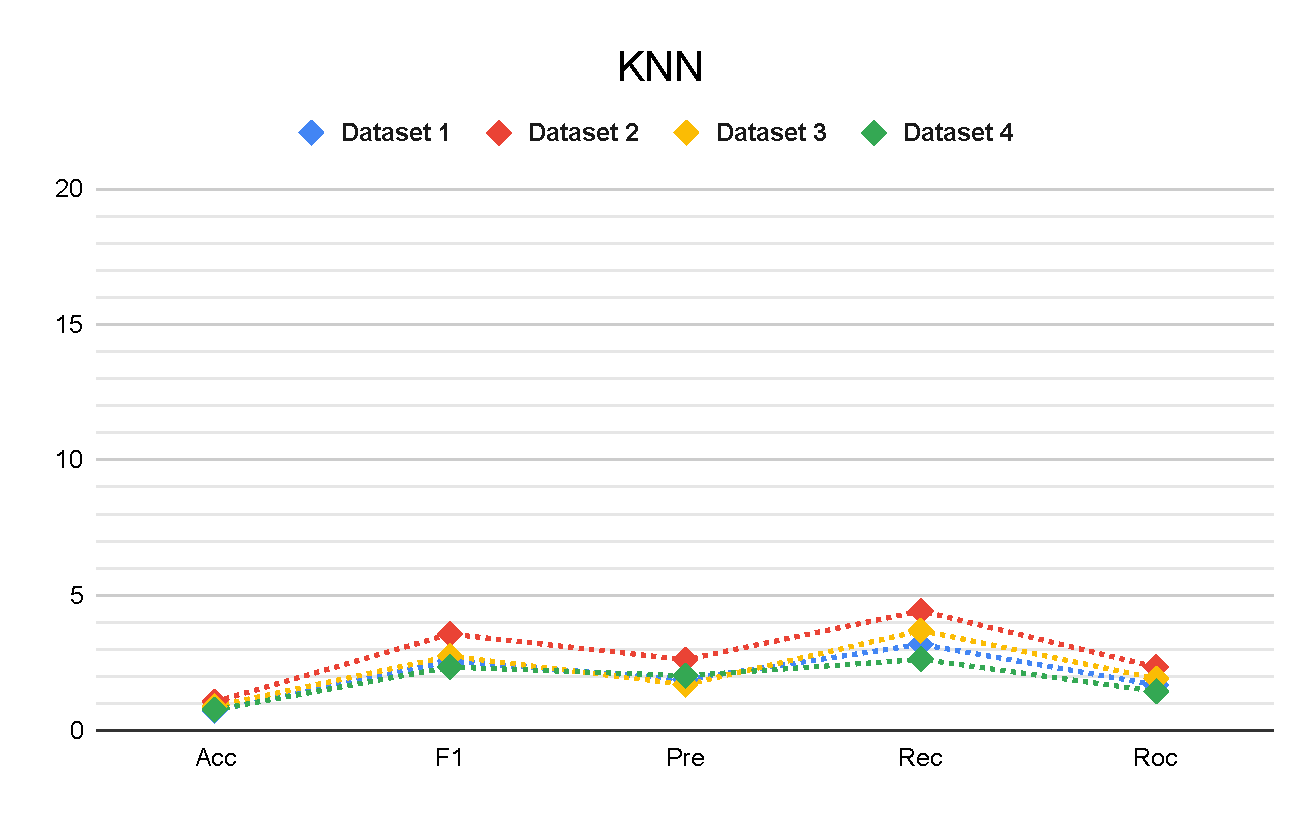
\includegraphics[width=0.9\columnwidth]{media/data/performance_delta/delta_KNN.pdf}
    \caption{}
    \label{fig:perfromance_delta_knn}
  \end{subfigure}%
  % ******************************************** DT *********************************************
  \begin{subfigure}{.5\columnwidth}
    \centering
    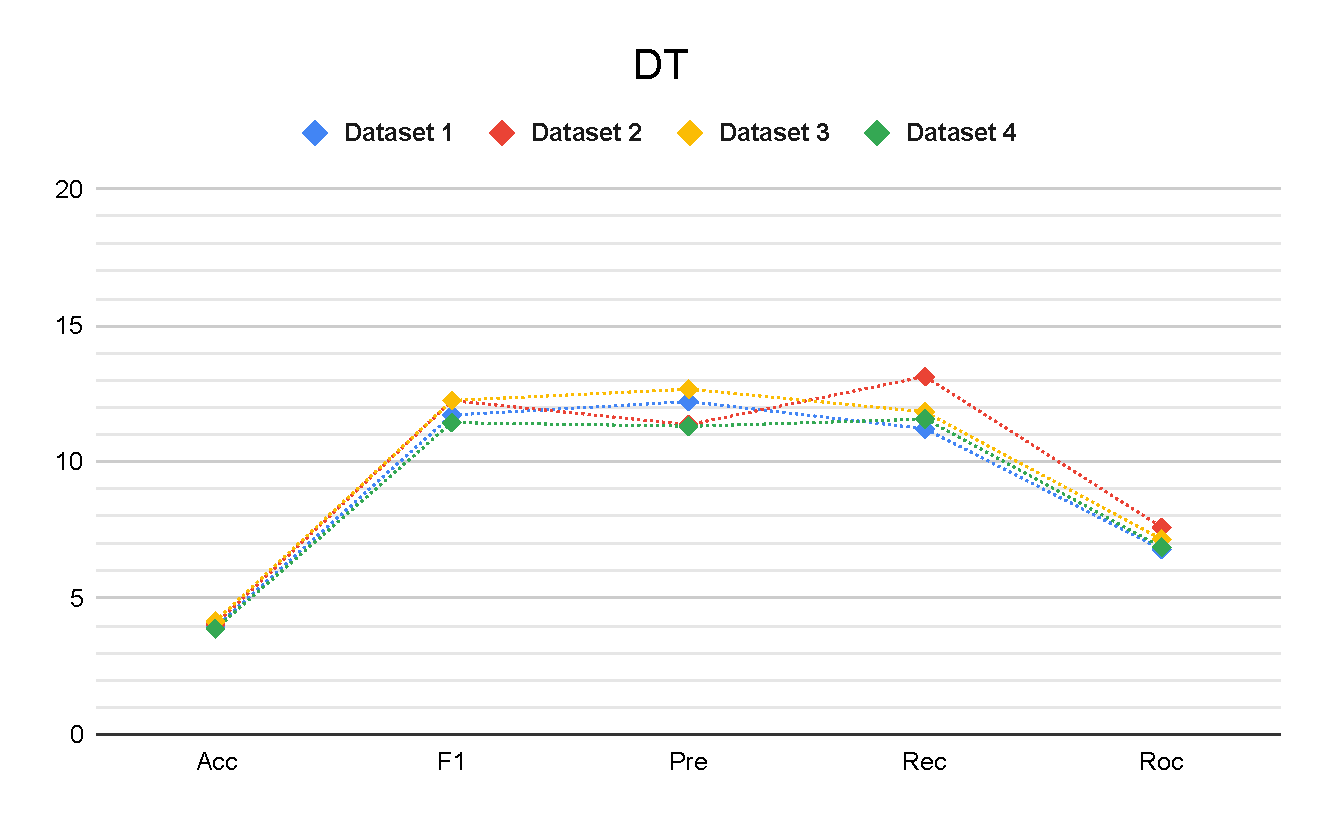
\includegraphics[width=0.9\columnwidth]{media/data/performance_delta/delta_DT.pdf}
    \caption{}
    \label{fig:perfromance_delta_dt}
  \end{subfigure}\\%
  % ******************************************** RF *********************************************
  \begin{subfigure}{.5\columnwidth}
    \centering
    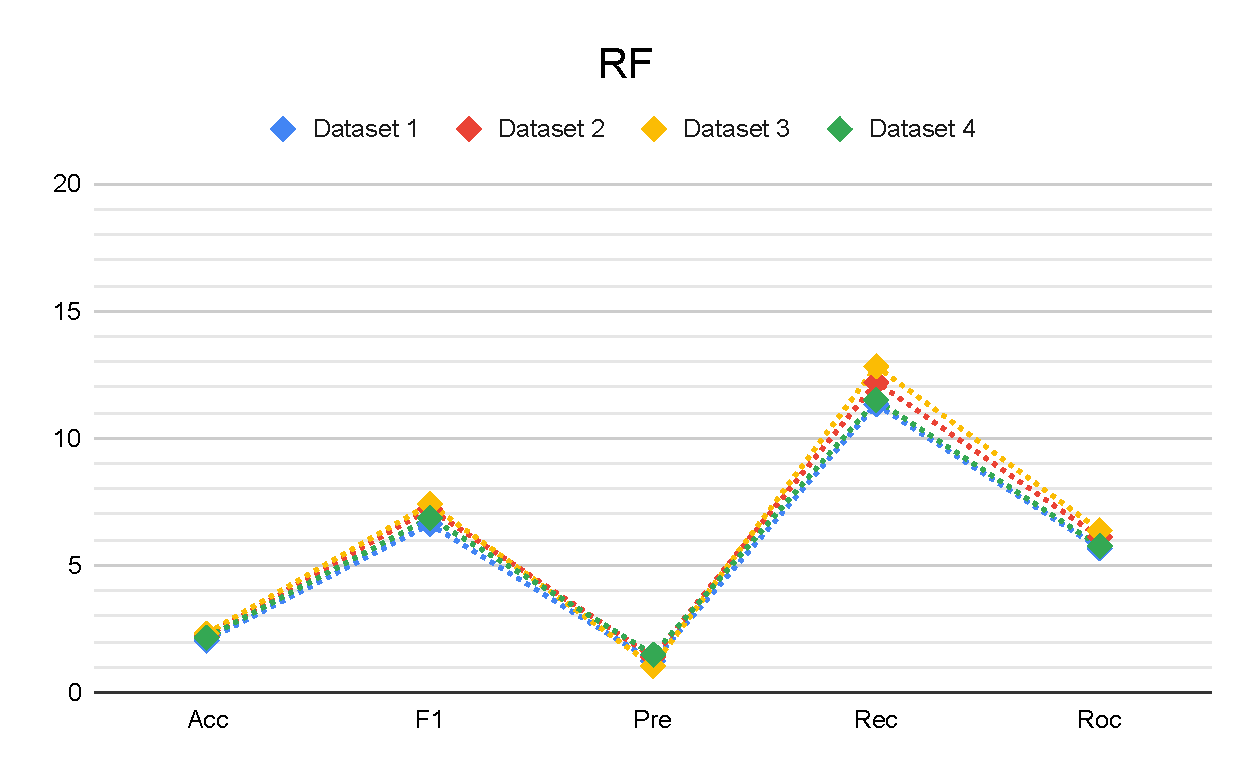
\includegraphics[width=0.9\columnwidth]{media/data/performance_delta/delta_RF.pdf}
    \caption{}
    \label{fig:perfromance_delta_rf}
  \end{subfigure}%
  % ******************************************** MLP ********************************************
  \begin{subfigure}{.5\columnwidth}
    \centering
    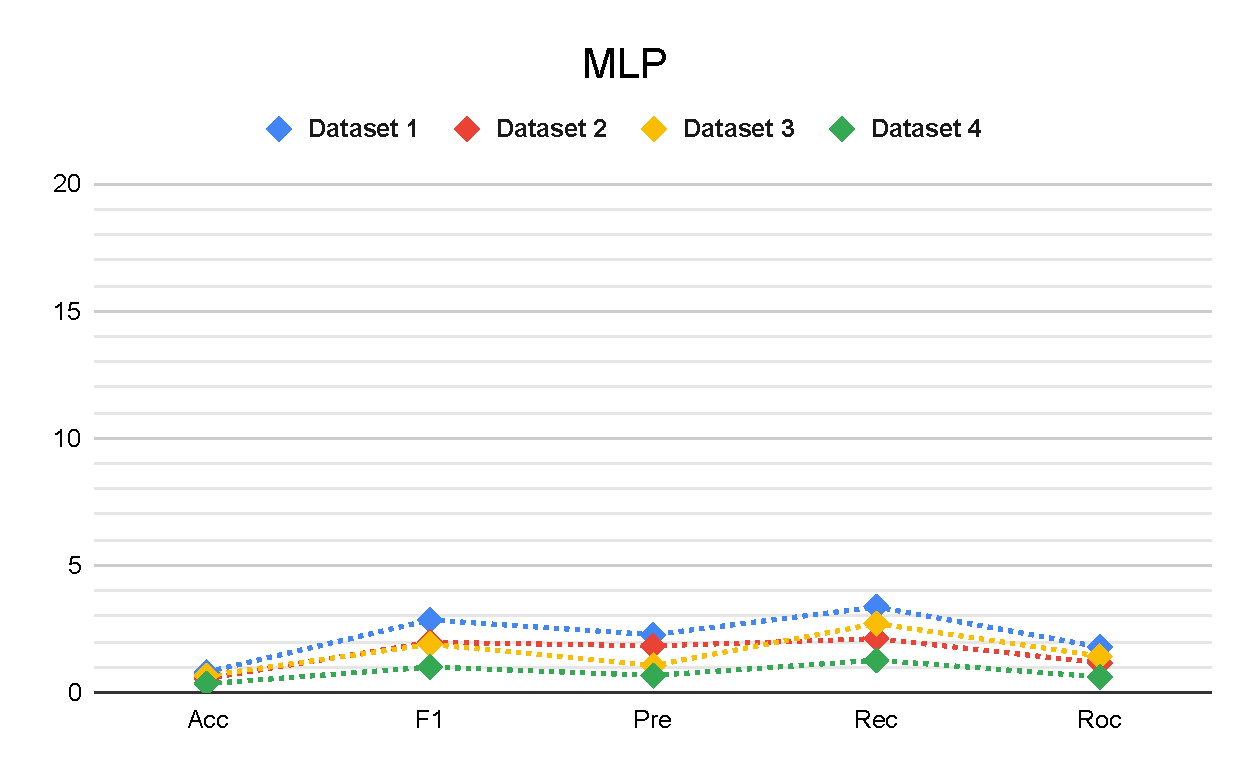
\includegraphics[width=0.9\columnwidth]{media/data/performance_delta/delta_MLP.pdf}
    \caption{}
    \label{fig:perfromance_delta_mlp}
  \end{subfigure}\\%
  % ******************************************** SVM ********************************************
  \begin{subfigure}{.5\columnwidth}
    \centering
    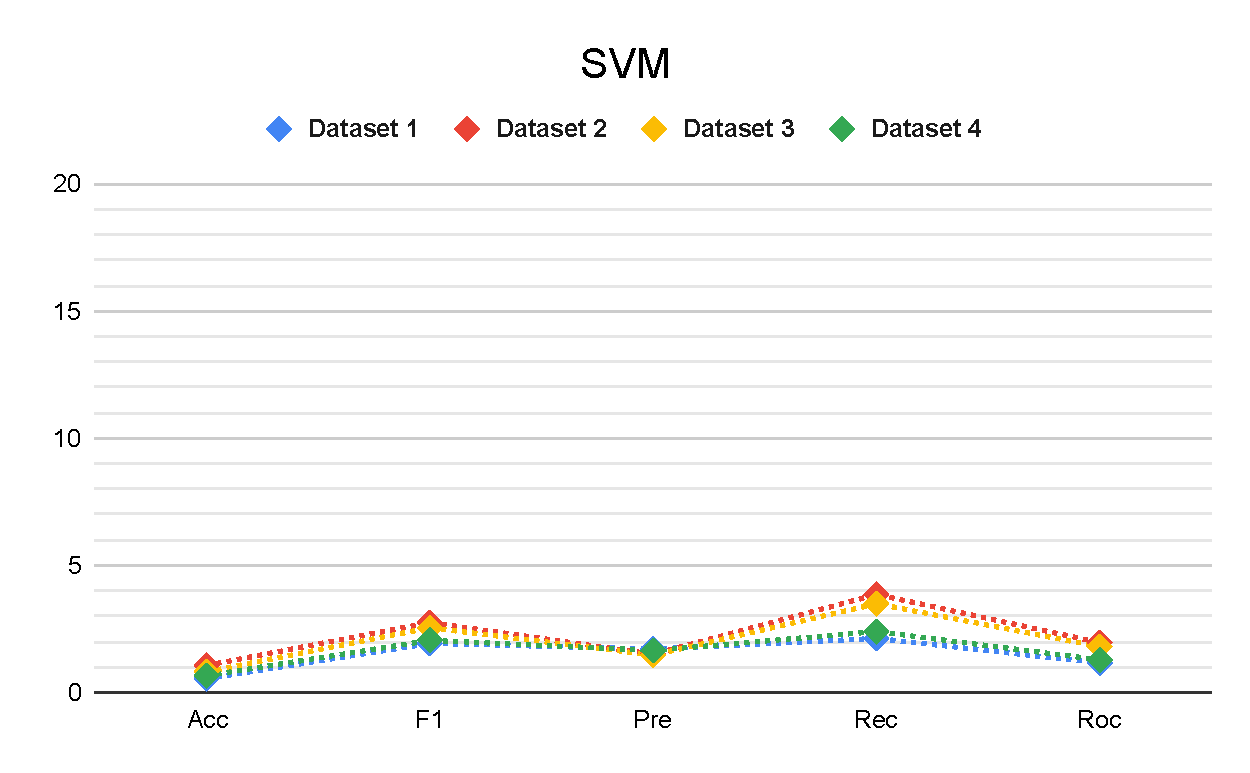
\includegraphics[width=0.9\columnwidth]{media/data/performance_delta/delta_SVM.pdf}
    \caption{}
    \label{fig:perfromance_delta_svm}
  \end{subfigure}
  \caption{Average Perfromance drop}
  \label{fig:perfromance_delta}
\end{figure}

The figure \ref{fig:perfromance_delta} shows the average performance difference of models concerning training datasets. From figure \ref{fig:perfromance_delta_dt} and \ref{fig:perfromance_delta_rf}, we can see that the difference in performance metrics of the Decision Tree and Random Forest algorithm is almost similar to all training sets. It indicates that these models can be used as solutions to similar problems. Figure \ref{fig:perfromance_delta_mlp} shows the maximum difference in performance metrics when tested against other datasets. It indicates that the model is overfitting and is not suitable to be used for other datasets. While figure \ref{fig:perfromance_delta_knn} and \ref{fig:perfromance_delta_svm} shows good performance metrics for some datasets. This shows models can be tuned for specific requirements. This will produce more satisfactory results in general predictions. Tables \ref{tab:dt_model_cross-performance_results}, \ref{tab:knn_model_cross-performance_results}, \ref{tab:mlp_model_cross-performance_results}, \ref{tab:rf_model_cross-performance_results} and \ref{tab:svm_model_cross-performance_results} shows the cross-performance evaluation of models.

% ********************************* cross performance tables **********************************
% ************************************** DT model table ***************************************
\begin{table}[H]
  \centering
  \caption{DT model cross-performance results}\label{tab:dt_model_cross-performance_results}
  \begin{subtable}[H]{0.45\textwidth}
    \centering
    \begin{tabular}{|l|c|c|c|c|}
      \hline
      \textbf{Dataset}   & \textbf{1} & \textbf{2} & \textbf{3} & \textbf{4} \\
      \hline
      \textbf{Accuracy}  & 0.98       & 0.94       & 0.94       & 0.94       \\
      \textbf{F1}        & 0.96       & 0.85       & 0.85       & 0.84       \\
      \textbf{Precision} & 0.95       & 0.83       & 0.84       & 0.83       \\
      \textbf{Recall}    & 0.96       & 0.86       & 0.85       & 0.85       \\
      \textbf{ROC}       & 0.97       & 0.91       & 0.91       & 0.90       \\
      \hline
    \end{tabular}
    \caption{Dataset 1 - DT Model}\label{subtab:dataset_1_dt_model}
  \end{subtable}
  \quad
  \begin{subtable}[H]{0.45\textwidth}
    \centering
    \begin{tabular}{|l|c|c|c|c|}
      \hline
      \textbf{Dataset}   & \textbf{1} & \textbf{2} & \textbf{3} & \textbf{4} \\
      \hline
      \textbf{Accuracy}  & 0.94       & 0.98       & 0.94       & 0.94       \\
      \textbf{F1}        & 0.84       & 0.96       & 0.84       & 0.85       \\
      \textbf{Precision} & 0.85       & 0.96       & 0.85       & 0.85       \\
      \textbf{Recall}    & 0.82       & 0.96       & 0.84       & 0.84       \\
      \textbf{ROC}       & 0.89       & 0.97       & 0.90       & 0.90       \\
      \hline
    \end{tabular}
    \caption{Dataset 2 - DT Model}\label{subtab:dataset_2_dt_model}
  \end{subtable}
  \quad
  \begin{subtable}[H]{0.45\textwidth}
    \centering
    \begin{tabular}{|l|c|c|c|c|}
      \hline
      \textbf{Dataset}   & \textbf{1} & \textbf{2} & \textbf{3} & \textbf{4} \\
      \hline
      \textbf{Accuracy}  & 0.94       & 0.94       & 0.98       & 0.94       \\
      \textbf{F1}        & 0.84       & 0.84       & 0.96       & 0.83       \\
      \textbf{Precision} & 0.84       & 0.83       & 0.95       & 0.83       \\
      \textbf{Recall}    & 0.84       & 0.85       & 0.96       & 0.84       \\
      \textbf{ROC}       & 0.90       & 0.90       & 0.97       & 0.90       \\
      \hline
    \end{tabular}
    \caption{Dataset 3 - DT Model}\label{subtab:dataset_3_dt_model}
  \end{subtable}
  \quad
  \begin{subtable}[H]{0.45\textwidth}
    \centering
    \begin{tabular}{|l|c|c|c|c|}
      \hline
      \textbf{Dataset}   & \textbf{1} & \textbf{2} & \textbf{3} & \textbf{4} \\
      \hline
      \textbf{Accuracy}  & 0.94       & 0.94       & 0.95       & 0.98       \\
      \textbf{F1}        & 0.85       & 0.85       & 0.85       & 0.96       \\
      \textbf{Precision} & 0.85       & 0.85       & 0.85       & 0.96       \\
      \textbf{Recall}    & 0.85       & 0.84       & 0.85       & 0.96       \\
      \textbf{ROC}       & 0.91       & 0.90       & 0.91       & 0.97       \\
      \hline
    \end{tabular}
    \caption{Dataset 4 - DT Model}\label{subtab:dataset_4_dt_model}
  \end{subtable}
\end{table}

% ************************************** KNN model table **************************************
\begin{table}[H]
  \centering
  \caption{KNN model cross-performance results}\label{tab:knn_model_cross-performance_results}
  \begin{subtable}[H]{0.45\textwidth}
    \centering
    \begin{tabular}{|l|c|c|c|c|}
      \hline
      \textbf{Dataset}   & \textbf{1} & \textbf{2} & \textbf{3} & \textbf{4} \\
      \hline
      \textbf{Accuracy}  & 0.97       & 0.97       & 0.97       & 0.96       \\
      \textbf{F1}        & 0.93       & 0.91       & 0.90       & 0.90       \\
      \textbf{Precision} & 0.96       & 0.95       & 0.94       & 0.94       \\
      \textbf{Recall}    & 0.90       & 0.87       & 0.87       & 0.87       \\
      \textbf{ROC}       & 0.94       & 0.93       & 0.93       & 0.93       \\
      \hline
    \end{tabular}
    \caption{Dataset 1 - KNN Model}\label{subtab:dataset_1_knn_model}
  \end{subtable}
  \quad
  \begin{subtable}[H]{0.45\textwidth}
    \centering
    \begin{tabular}{|l|c|c|c|c|}
      \hline
      \textbf{Dataset}   & \textbf{1} & \textbf{2} & \textbf{3} & \textbf{4} \\
      \hline
      \textbf{Accuracy}  & 0.96       & 0.97       & 0.96       & 0.96       \\
      \textbf{F1}        & 0.90       & 0.93       & 0.90       & 0.89       \\
      \textbf{Precision} & 0.94       & 0.96       & 0.94       & 0.94       \\
      \textbf{Recall}    & 0.86       & 0.90       & 0.86       & 0.85       \\
      \textbf{ROC}       & 0.92       & 0.94       & 0.92       & 0.92       \\
      \hline
    \end{tabular}
    \caption{Dataset 2 - KNN Model}\label{subtab:dataset_2_knn_model}
  \end{subtable}
  \quad
  \begin{subtable}[H]{0.45\textwidth}
    \centering
    \begin{tabular}{|l|c|c|c|c|}
      \hline
      \textbf{Dataset}   & \textbf{1} & \textbf{2} & \textbf{3} & \textbf{4} \\
      \hline
      \textbf{Accuracy}  & 0.96       & 0.96       & 0.97       & 0.96       \\
      \textbf{F1}        & 0.90       & 0.90       & 0.93       & 0.90       \\
      \textbf{Precision} & 0.95       & 0.95       & 0.96       & 0.94       \\
      \textbf{Recall}    & 0.86       & 0.86       & 0.89       & 0.86       \\
      \textbf{ROC}       & 0.92       & 0.92       & 0.94       & 0.92       \\
      \hline
    \end{tabular}
    \caption{Dataset 3 - KNN Model}\label{subtab:dataset_3_knn_model}
  \end{subtable}
  \quad
  \begin{subtable}[H]{0.45\textwidth}
    \centering
    \begin{tabular}{|l|c|c|c|c|}
      \hline
      \textbf{Dataset}   & \textbf{1} & \textbf{2} & \textbf{3} & \textbf{4} \\
      \hline
      \textbf{Accuracy}  & 0.96       & 0.96       & 0.96       & 0.97       \\
      \textbf{F1}        & 0.90       & 0.90       & 0.90       & 0.92       \\
      \textbf{Precision} & 0.94       & 0.95       & 0.94       & 0.96       \\
      \textbf{Recall}    & 0.86       & 0.86       & 0.87       & 0.89       \\
      \textbf{ROC}       & 0.92       & 0.92       & 0.93       & 0.94       \\
      \hline
    \end{tabular}
    \caption{Dataset 4 - KNN Model}\label{subtab:dataset_4_knn_model}
  \end{subtable}
\end{table}

% ************************************** MLP model table **************************************
\begin{table}[H]
  \centering
  \caption{MLP model cross-performance results}\label{tab:mlp_model_cross-performance_results}
  \begin{subtable}[H]{0.45\textwidth}
    \centering
    \begin{tabular}{|l|c|c|c|c|}
      \hline
      \textbf{Dataset}   & \textbf{1} & \textbf{2} & \textbf{3} & \textbf{4} \\
      \hline
      \textbf{Accuracy}  & 0.97       & 0.96       & 0.96       & 0.96       \\
      \textbf{F1}        & 0.92       & 0.89       & 0.89       & 0.89       \\
      \textbf{Precision} & 0.97       & 0.95       & 0.94       & 0.95       \\
      \textbf{Recall}    & 0.88       & 0.85       & 0.85       & 0.85       \\
      \textbf{ROC}       & 0.93       & 0.92       & 0.92       & 0.92       \\
      \hline
    \end{tabular}
    \caption{Dataset 1 - MLP Model}\label{subtab:dataset_1_mlp_model}
  \end{subtable}
  \quad
  \begin{subtable}[H]{0.45\textwidth}
    \centering
    \begin{tabular}{|l|c|c|c|c|}
      \hline
      \textbf{Dataset}   & \textbf{1} & \textbf{2} & \textbf{3} & \textbf{4} \\
      \hline
      \textbf{Accuracy}  & 0.96       & 0.97       & 0.96       & 0.96       \\
      \textbf{F1}        & 0.90       & 0.91       & 0.90       & 0.90       \\
      \textbf{Precision} & 0.95       & 0.97       & 0.94       & 0.95       \\
      \textbf{Recall}    & 0.85       & 0.87       & 0.85       & 0.85       \\
      \textbf{ROC}       & 0.92       & 0.93       & 0.92       & 0.92       \\
      \hline
    \end{tabular}
    \caption{Dataset 2 - MLP Model}\label{subtab:dataset_2_mlp_model}
  \end{subtable}
  \quad
  \begin{subtable}[H]{0.45\textwidth}
    \centering
    \begin{tabular}{|l|c|c|c|c|}
      \hline
      \textbf{Dataset}   & \textbf{1} & \textbf{2} & \textbf{3} & \textbf{4} \\
      \hline
      \textbf{Accuracy}  & 0.96       & 0.96       & 0.96       & 0.96       \\
      \textbf{F1}        & 0.89       & 0.89       & 0.90       & 0.88       \\
      \textbf{Precision} & 0.89       & 0.89       & 0.90       & 0.89       \\
      \textbf{Recall}    & 0.88       & 0.88       & 0.91       & 0.88       \\
      \textbf{ROC}       & 0.93       & 0.93       & 0.94       & 0.93       \\
      \hline
    \end{tabular}
    \caption{Dataset 3 - MLP Model}\label{subtab:dataset_3_mlp_model}
  \end{subtable}
  \quad
  \begin{subtable}[H]{0.45\textwidth}
    \centering
    \begin{tabular}{|l|c|c|c|c|}
      \hline
      \textbf{Dataset}   & \textbf{1} & \textbf{2} & \textbf{3} & \textbf{4} \\
      \hline
      \textbf{Accuracy}  & 0.95       & 0.95       & 0.95       & 0.95       \\
      \textbf{F1}        & 0.85       & 0.85       & 0.85       & 0.86       \\
      \textbf{Precision} & 0.97       & 0.97       & 0.97       & 0.98       \\
      \textbf{Recall}    & 0.75       & 0.75       & 0.75       & 0.76       \\
      \textbf{ROC}       & 0.87       & 0.87       & 0.87       & 0.88       \\
      \hline
    \end{tabular}
    \caption{Dataset 4 - MLP Model}\label{subtab:dataset_4_mlp_model}
  \end{subtable}
\end{table}

% ************************************** RF model table **************************************
\begin{table}[H]
  \centering
  \caption{RF model cross-performance results}\label{tab:rf_model_cross-performance_results}
  \begin{subtable}[H]{0.45\textwidth}
    \centering
    \begin{tabular}{|l|c|c|c|c|}
      \hline
      \textbf{Dataset}   & \textbf{1} & \textbf{2} & \textbf{3} & \textbf{4} \\
      \hline
      \textbf{Accuracy}  & 0.99       & 0.97       & 0.97       & 0.97       \\
      \textbf{F1}        & 0.98       & 0.91       & 0.91       & 0.91       \\
      \textbf{Precision} & 0.99       & 0.98       & 0.97       & 0.98       \\
      \textbf{Recall}    & 0.96       & 0.85       & 0.85       & 0.85       \\
      \textbf{ROC}       & 0.98       & 0.92       & 0.92       & 0.92       \\
      \hline
    \end{tabular}
    \caption{Dataset 1 - RF Model}\label{subtab:dataset_1_rf_model}
  \end{subtable}
  \quad
  \begin{subtable}[H]{0.45\textwidth}
    \centering
    \begin{tabular}{|l|c|c|c|c|}
      \hline
      \textbf{Dataset}   & \textbf{1} & \textbf{2} & \textbf{3} & \textbf{4} \\
      \hline
      \textbf{Accuracy}  & 0.96       & 0.99       & 0.97       & 0.97       \\
      \textbf{F1}        & 0.90       & 0.97       & 0.91       & 0.90       \\
      \textbf{Precision} & 0.98       & 0.99       & 0.97       & 0.98       \\
      \textbf{Recall}    & 0.83       & 0.96       & 0.85       & 0.84       \\
      \textbf{ROC}       & 0.91       & 0.98       & 0.92       & 0.91       \\
      \hline
    \end{tabular}
    \caption{Dataset 2 - RF Model}\label{subtab:dataset_2_rf_model}
  \end{subtable}
  \quad
  \begin{subtable}[H]{0.45\textwidth}
    \centering
    \begin{tabular}{|l|c|c|c|c|}
      \hline
      \textbf{Dataset}   & \textbf{1} & \textbf{2} & \textbf{3} & \textbf{4} \\
      \hline
      \textbf{Accuracy}  & 0.96       & 0.97       & 0.99       & 0.97       \\
      \textbf{F1}        & 0.90       & 0.90       & 0.97       & 0.90       \\
      \textbf{Precision} & 0.98       & 0.98       & 0.99       & 0.98       \\
      \textbf{Recall}    & 0.83       & 0.84       & 0.96       & 0.83       \\
      \textbf{ROC}       & 0.91       & 0.91       & 0.98       & 0.91       \\
      \hline
    \end{tabular}
    \caption{Dataset 3 - RF Model}\label{subtab:dataset_3_rf_model}
  \end{subtable}
  \quad
  \begin{subtable}[H]{0.45\textwidth}
    \centering
    \begin{tabular}{|l|c|c|c|c|}
      \hline
      \textbf{Dataset}   & \textbf{1} & \textbf{2} & \textbf{3} & \textbf{4} \\
      \hline
      \textbf{Accuracy}  & 0.96       & 0.97       & 0.97       & 0.99       \\
      \textbf{F1}        & 0.90       & 0.91       & 0.90       & 0.97       \\
      \textbf{Precision} & 0.98       & 0.98       & 0.97       & 0.99       \\
      \textbf{Recall}    & 0.84       & 0.84       & 0.85       & 0.95       \\
      \textbf{ROC}       & 0.91       & 0.92       & 0.92       & 0.97       \\
      \hline
    \end{tabular}
    \caption{Dataset 4 - RF Model}\label{subtab:dataset_4_rf_model}
  \end{subtable}
\end{table}

% ************************************** SVM model table **************************************
\begin{table}[H]
  \centering
  \caption{SVM model cross-performance results}\label{tab:svm_model_cross-performance_results}
  \begin{subtable}[H]{0.45\textwidth}
    \centering
    \begin{tabular}{|l|c|c|c|c|}
      \hline
      \textbf{Dataset}   & \textbf{1} & \textbf{2} & \textbf{3} & \textbf{4} \\
      \hline
      \textbf{Accuracy}  & 0.97       & 0.97       & 0.97       & 0.97       \\
      \textbf{F1}        & 0.93       & 0.92       & 0.91       & 0.91       \\
      \textbf{Precision} & 0.98       & 0.97       & 0.96       & 0.96       \\
      \textbf{Recall}    & 0.89       & 0.87       & 0.87       & 0.87       \\
      \textbf{ROC}       & 0.94       & 0.93       & 0.93       & 0.93       \\
      \hline
    \end{tabular}
    \caption{Dataset 1 - SVM Model}\label{subtab:dataset_1_svm_model}
  \end{subtable}
  \quad
  \begin{subtable}[H]{0.45\textwidth}
    \centering
    \begin{tabular}{|l|c|c|c|c|}
      \hline
      \textbf{Dataset}   & \textbf{1} & \textbf{2} & \textbf{3} & \textbf{4} \\
      \hline
      \textbf{Accuracy}  & 0.97       & 0.98       & 0.97       & 0.97       \\
      \textbf{F1}        & 0.91       & 0.94       & 0.91       & 0.91       \\
      \textbf{Precision} & 0.97       & 0.98       & 0.96       & 0.96       \\
      \textbf{Recall}    & 0.86       & 0.89       & 0.86       & 0.86       \\
      \textbf{ROC}       & 0.92       & 0.94       & 0.93       & 0.92       \\
      \hline
    \end{tabular}
    \caption{Dataset 2 - SVM Model}\label{subtab:dataset_2_svm_model}
  \end{subtable}
  \quad
  \begin{subtable}[H]{0.45\textwidth}
    \centering
    \begin{tabular}{|l|c|c|c|c|}
      \hline
      \textbf{Dataset}   & \textbf{1} & \textbf{2} & \textbf{3} & \textbf{4} \\
      \hline
      \textbf{Accuracy}  & 0.97       & 0.97       & 0.98       & 0.97       \\
      \textbf{F1}        & 0.91       & 0.92       & 0.94       & 0.91       \\
      \textbf{Precision} & 0.97       & 0.97       & 0.98       & 0.97       \\
      \textbf{Recall}    & 0.85       & 0.87       & 0.89       & 0.87       \\
      \textbf{ROC}       & 0.92       & 0.93       & 0.94       & 0.93       \\
      \hline
    \end{tabular}
    \caption{Dataset 3 - SVM Model}\label{subtab:dataset_3_svm_model}
  \end{subtable}
  \quad
  \begin{subtable}[H]{0.45\textwidth}
    \centering
    \begin{tabular}{|l|c|c|c|c|}
      \hline
      \textbf{Dataset}   & \textbf{1} & \textbf{2} & \textbf{3} & \textbf{4} \\
      \hline
      \textbf{Accuracy}  & 0.97       & 0.97       & 0.97       & 0.97       \\
      \textbf{F1}        & 0.91       & 0.91       & 0.91       & 0.93       \\
      \textbf{Precision} & 0.97       & 0.96       & 0.96       & 0.98       \\
      \textbf{Recall}    & 0.85       & 0.86       & 0.86       & 0.88       \\
      \textbf{ROC}       & 0.92       & 0.93       & 0.93       & 0.94       \\
      \hline
    \end{tabular}
    \caption{Dataset 4 - SVM Model}\label{subtab:dataset_4_svm_model}
  \end{subtable}
\end{table}

% *********************************************************************************************
% ******************************* Discarded code for future use *******************************
% *********************************************************************************************
%
% ************************************** model peformance *************************************
%
% \begin{table}[H]
%     \centering
%     \caption{Performance of models trained on following datasets}\label{tab:performance_of_models_trained_on_following_datasets}
%         \begin{subtable}[H]{0.9\textwidth}
%             \centering
%             \begin{tabular}{|p{5em}|C{3em}|C{3em}|C{3em}|C{3em}|C{3em}|}
%                 \hline
%                 \textbf{Metric} & \textbf{KNN} & \textbf{DT} & \textbf{MLP} & \textbf{RF} & \textbf{SVM} \\
%                 \hline
%                 \textbf{Accuracy} & 96.72 & 94.46 & 96.89 & 97.33 & \textbf{97.40} \\
%                 \textbf{F1} & 89.71 & 83.43 & 90.05 & 91.30 & \textbf{91.69} \\
%                 \textbf{Precision} & 92.53 & 81.86 & 94.71 & 97.95 & \textbf{96.43} \\
%                 \textbf{Recall} & 87.06 & 85.06 & 85.84 & 85.50 & \textbf{87.40} \\
%                 \textbf{ROC} & 92.84 & 90.68 & 92.45 & 92.57 & \textbf{93.38} \\
%                 \textbf{Time(s)} & 0.457 & 0.001 & 0.002 & 0.015 & \textbf{0.297} \\
%                 \hline
%             \end{tabular}
%             \caption{Dataset 1}\label{tab:performance_of_models_trained_on_dataset_1}
%         \end{subtable}
%     \begin{subtable}[H]{0.9\textwidth}
%         \centering
%         \begin{tabular}{|p{5em}|C{3em}|C{3em}|C{3em}|C{3em}|C{3em}|}
%             \hline
%             \textbf{Metric} & \textbf{KNN} & \textbf{DT} & \textbf{MLP} & \textbf{RF} & \textbf{SVM} \\
%             \hline
%             \textbf{Accuracy} & 96.83 & 95.04 & 96.69 & 97.09 & \textbf{97.46} \\
%             \textbf{F1} & 90.28 & 85.50 & 89.73 & 90.75 & \textbf{92.15} \\
%             \textbf{Precision} & 94.25 & 84.90 & 94.73 & 98.60 & \textbf{96.79} \\
%             \textbf{Recall} & 86.63 & 86.09 & 85.23 & 84.05 & \textbf{87.93} \\
%             \textbf{ROC} & 92.77 & 91.48 & 92.13 & 91.90 & \textbf{93.66} \\
%             \textbf{Time(s)} & 0.435 & 0.001 & 0.003 & 0.014 & \textbf{0.295} \\
%             \hline
%         \end{tabular}
%         \caption{Dataset 2}\label{subtab:models_trained_on_dataset_2}
%     \end{subtable}
%     \quad
%     \begin{subtable}[H]{0.9\textwidth}
%         \centering
%         \begin{tabular}{|p{5em}|C{3em}|C{3em}|C{3em}|C{3em}|C{3em}|}
%             \hline
%             \textbf{Metric} & \textbf{KNN} & \textbf{DT} & \textbf{MLP} & \textbf{RF} & \textbf{SVM} \\
%             \hline
%             \textbf{Accuracy} & 97.07 & 94.64 & 96.41 & \textbf{97.22} & 97.44 \\
%             \textbf{F1} & 90.93 & 84.30 & 89.34 & \textbf{91.21} & 92.00 \\
%             \textbf{Precision} & 95.82 & 83.81 & 90.13 & \textbf{98.37} & 97.81 \\
%             \textbf{Recall} & 86.53 & 84.80 & 88.57 & \textbf{85.02} & 86.85 \\
%             \textbf{ROC} & 92.87 & 90.73 & 93.29 & \textbf{92.36} & 93.22 \\
%             \textbf{Time(s)} & 0.404 & 0.001 & 0.002 & \textbf{0.017} & 0.293 \\
%             \hline
%         \end{tabular}
%         \caption{Dataset 3}\label{subtab:models_trained_on_dataset_3}
%     \end{subtable}
%     \quad
%     \begin{subtable}[H]{0.9\textwidth}
%         \centering
%         \begin{tabular}{|p{5em}|C{3em}|C{3em}|C{3em}|C{3em}|C{3em}|}
%             \hline
%             \textbf{Metric} & \textbf{KNN} & \textbf{DT} & \textbf{MLP} & \textbf{RF} & \textbf{SVM} \\
%             \hline
%             \textbf{Accuracy} & 96.84 & 94.99 & 95.34 & 96.88 & \textbf{97.15} \\
%             \textbf{F1} & 90.52 & 85.73 & 85.01 & 90.37 & \textbf{91.39} \\
%             \textbf{Precision} & 95.71 & 85.91 & 97.83 & 98.65 & \textbf{97.41} \\
%             \textbf{Recall} & 85.86 & 85.55 & 75.15 & 83.37 & \textbf{86.07} \\
%             \textbf{ROC} & 92.52 & 91.28 & 87.40 & 91.56 & \textbf{92.79} \\
%             \textbf{Time(s)} & 0.452 & 0.001 & 0.002 & 0.014 & \textbf{0.294} \\
%             \hline
%         \end{tabular}
%         \caption{Dataset 4}\label{subtab:models_trained_on_dataset_4}
%     \end{subtable}
% \end{table}
%
% ******************************************** End ********************************************